\documentclass[11pt,a4paper,titlepage]{article}
\usepackage[pdftex]{graphicx}
\usepackage{listings}
\usepackage{titlesec}
\usepackage{float}
\usepackage{enumitem}
\usepackage{color}
\usepackage{pdflscape}
\usepackage{hyperref}
\hypersetup{
	colorlinks,
	citecolor=black,
	filecolor=black,
	linkcolor=black,
	urlcolor=black
}

\definecolor{dkgreen}{rgb}{0,0.6,0}
\definecolor{gray}{rgb}{0.5,0.5,0.5}
\definecolor{mauve}{rgb}{0.58,0,0.82}

\lstdefinelanguage{Alloy}{
	keywords={%
		assert, pred, all, no, lone, one, some, check, run,
		but, let, implies, not, iff, in, and, or, set, sig, Int, int,
		if, then, else, exactly, disj, fact, fun, module, abstract,
		extends, open, none, univ, iden, seq,
	},
	literate=%
	{:}{$\colon$}1
	{==}{$=$}1
	{=}{$=$}1
	{!=}{$\neq$}1
	{&&}{$\land$}1
	{||}{$\lor$}1
	{<=}{$\le$}1
	{>=}{$\ge$}1
	{all}{$\forall$}1
	{exists}{$\exists$}1
	{!in}{$\not\in$}1
	{\\in}{$\in$}1
	{=>}{$\implies$}2
	% the following isn't actually Alloy, but it gives the option to produce nicer latex
	{|=>}{$\Rightarrow$}2
	{<=set}{$\subseteq$}1
	{+set}{$\cup$}1
	{*set}{$\cap$}1
	{==>}{$\Longrightarrow$}3
	{<==>}{$\Longleftrightarrow$}4
	{...}{$\ldots$}1
	{\\hl}{$\hline$}1
	{\\alpha}{$\alpha$}1
	{\\beta}{$\beta$}1
	{\\gamma}{$\gamma$}1
	{\\delta}{$\delta$}1
	{\\epsilon}{$\epsilon$}1
	{\\zeta}{$\zeta$}1
	{\\eta}{$\eta$}1
	{\\theta}{$\theta$}1
	{\\iota}{$\iota$}1
	{\\kappa}{$\kappa$}1
	{\\lambda}{$\lambda$}1
	{\\mu}{$\mu$}1
	{\\nu}{$\nu$}1
	{\\xi}{$\xi$}1
	{\\pi}{$\pi$}1
	{\\rho}{$\rho$}1
	{\\sigma}{$\sigma$}1
	{\\tau}{$\tau$}1
	{\\upsilon}{$\upsilon$}1
	{\\phi}{$\phi$}1
	{\\chi}{$\chi$}1
	{\\psi}{$\psi$}1
	{\\omega}{$\omega$}1
	{\\Gamma}{$\Gamma$}1
	{\\Delta}{$\Delta$}1
	{\\Theta}{$\Theta$}1
	{\\Lambda}{$\Lambda$}1
	{\\Xi}{$\Xi$}1
	{\\Pi}{$\Pi$}1
	{\\Sigma}{$\Sigma$}1
	{\\Upsilon}{$\Upsilon$}1
	{\\Phi}{$\Phi$}1
	{\\Psi}{$\Psi$}1
	{\\Omega}{$\Omega$}1
	{\\EOF}{\;}1
	,
	sensitive=true,  % case sensitive
	morecomment=[l]//,%
	morecomment=[l]{--},%
	morecomment=[s]{/*}{*/},%
	morestring=[b]",
	numbers=none,
	firstnumber=1,
	numberstyle=\tiny\color{gray},
	stepnumber=2,
	basicstyle=\scriptsize,
	commentstyle=\itshape\color{dkgreen},
	keywordstyle=\bfseries\color{blue},
	ndkeywordstyle=\bfseries,
	stringstyle=\color{mauve},
	breaklines=true,
	breakatwhitespace=true,
	tabsize=3
}

% inline
\def\A{%
	\lstinline[language=alloy,basicstyle=\ttfamily,columns=fixed]}

% paragraph
\lstnewenvironment{alloy}[1][]{%
	\lstset{language=alloy,
		floatplacement={tbp},captionpos=b,
		xleftmargin=8pt,xrightmargin=8pt,basicstyle=\ttfamily,#1}}{}

% paragraph from file
\newcommand{\alloyfile}[1]{
	\lstinputlisting[language=alloy,%
	frame=lines,xleftmargin=8pt,xrightmargin=8pt,basicstyle=\ttfamily,columns=fixed]{#1}
}

\setcounter{secnumdepth}{4}

\titleformat{\paragraph}
{\normalfont\normalsize\bfseries}{\theparagraph}{1em}{}
\titlespacing*{\paragraph}
{0pt}{3.25ex plus 1ex minus .2ex}{1.5ex plus .2ex}

\begin{document}
\begin{figure}
	\centering
	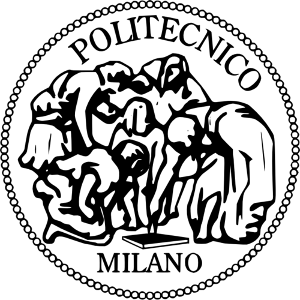
\includegraphics[scale=0.6]{../SE2_IMAGES/Logo_Politecnico_Milano}
\end{figure}
\title{Politecnico di Milano\\A.Y. 2015/2016\\\textbf{My Taxi Service}\\Requirement Analysis and Specification Document\\}
\author{Bernardis Cesare matr. 852509 \and Dagrada Mattia matr.852975}
\date{November 6, 2015}
\maketitle

\newpage

\tableofcontents

\newpage

\section{Introduction}
\subsection{Purpose}
The main goal of this document is to completely describe the system in terms of functional and non-functional requirements, to analyse the real need of the customer modelling the system, to show the constraints and the software limits and simulate the typical use cases that will occur after the development. This document is intended to all developers and programmers who have to implement the requirements, to the system analysts who want to integrate other system with this one, and could also be used as a contractual basis between the customer and the developer.
\subsection{Actual system}
The government of a large city wants to optimize its taxi service. We suppose that the actual taxi service is based on simple phone calls from customers to the taxi's call centre.
\subsection{Scope}
The aim of this project is to create a brand new taxi application that is used by both the taxi drivers and the passengers to access the taxi service. Passengers can access the service either via mobile or web application. They can request a taxi without having to register to service but they have to insert personal information while registered passengers, once logged in, can directly request a taxi. The system confirms a taxi request by sending the passenger the taxi code only when a taxi is found and an estimated arrival time. Registered passengers can also make taxi reservations and they will receive the code as soon as a taxi is found available. Taxi drivers can access the service only from mobile application. Once logged in they can give the system their availability, or revoke it, and they will receive from the system ride requests that they can either accept or refuse. The login interface of the application is shared by passengers and taxi drivers.
The system has the city map divided into areas of 2km$^{2}$ and holds a taxi queue in each area. It receives GPS coordinates from taxis, it assigns them to their corresponding area queue, placing them in the last position. Following a FIFO (First In First Out) logic, the first taxi receives a request and is then removed from the queue. In case of rejection, the taxi is placed in the last position of the queue.
\subsection{Actors}
\begin{description}
	\item[Guest] a guest is able to request a taxi without having to be registered to the service, but simply adding some essential personal information. A guest can register to the service filling in a registration form, becoming a Registered Passenger.
	\item[Registered Passenger] a registered passenger, once logged in, is able to request a taxi without having to add additional personal information. A registered passenger can also make reservations, specifying origin and destination of the ride, at least 2 hours before the desired time for the ride.
	\item[Taxi Drivers] a taxi driver, once logged in, has a different user interface than registered user, from which he will receive ride requests that he can accept or refuse. He will also be able to give his availability, which means that he is willing to pick up ride requests.
\end{description}
\subsection{Goals}
These are the goals of MyTaxiService application:
\begin{itemize}
	\item Permit a guest to register to the service.
	\item Permit a guest to request a taxi.
	\item Permit a guest to sign in and become a registered passenger
	\item Permit a registered passenger to require a taxi.
	\item Permit a registered passenger to make a reservation.
	\item Permit a registered passenger to cancel a reservation.
	\item Permit a taxi driver to give the system his availability.
	\item Permit a taxi driver to revoke his availability.
	\item Permit a taxi driver to accept a ride request.
	\item Permit a taxi driver to refuse a ride request.
\end{itemize}
\subsection{Reference Documents}
\begin{itemize}
	\item Specification Document: MyTaxiService Project A.Y.2015-2016.
	\item IEEE Std 830-1998 IEEE Recommended Practice for Software Requirements Specifications.
\end{itemize}
\subsection{Document overview}
This document is structured as following:
\begin{enumerate}
	\item \textbf{Introduction}: this section represents a generic description of the project, highlighting actors and goals.
	\item \textbf{Overall Description}: this section gives further informations about the project, focusing more on what are the assumptions made about the software and its constraints.
	\item \textbf{Specific Requirements}: this section lists the requirements of the software, both functional and non-functional ones. There are also some typical scenarios and use cases related to sequence diagrams along with a class diagram.
	\item \textbf{Alloy Modelling}: this section contains Alloy code and Alloy worlds.
	\item \textbf{Appendix}: this section contains extra information and also which software and tools has been used to write this document.
\end{enumerate}
\section{Overall Description}
	\subsection{Product perspective}
		We want to release both a web and a mobile application, avoiding deep
		integrations with other existing systems in order to keep an high level
		of compatibility, especially the mobile application, that we want to
		release for all major mobile operative systems. The applications will not
		have any internal interface for administration but they will be only user based.
		The application will provide APIs for a faster, safer and better integrated 
		implementation of new features, based on the basic functionalities
		offered by the system.
	\subsection{User characteristics}
		We expect to have two different types of user with distinct experiences. 
		\begin{description}
			\item[Passenger] who needs to call a taxi for a ride (that is occasional, threated
			as a guest, or habitual, who can register himself to speed up request submissions).
			This user must have access to the Internet and be able to use
			a web browser or have installed our mobile application on his smartphone;
			\item[Taxi Driver] who wants to offer its service through our system.
			This user must have access to Internet and have	installed our mobile
			application on his smartphone.
		\end{description}
	\subsection{Constraints}
		\subsubsection{Regulatory policies}
			Personal information (locations included) obtained from the	user will be stored
			in our databases if strictly necessary, to provide the best possible experience
			with our service. No information will be disclosed to any other company or
			used for any other purpose.
		\subsubsection{Hardware limitations}
			MyTaxiService's web application will be available on every device with an Internet
			connection and a browser installed. The mobile application (necessary for taxi
			drivers) will have the following requirements:
			\begin{itemize}
				\item 256MB total RAM
				\item 50MB of free space on Disk
				\item Internet Connection
				\item Operative System:
					\begin{itemize}
						\item Android 2.3 ''Gingerbread'' or later
						\item Windows Mobile 7.0 or later
						\item iOS 6.0 or later
					\end{itemize} 
			\end{itemize}
			It is also recommended to activate the GPS for a optimal localization.
		\subsubsection{Interfaces to other applications}
			MyTaxiService will provide an API library to allow external developers to
			integrate their applications with our system.
		\subsubsection{Parallel operation}
			The system must support parallel operations from different users. Information
			integrity is fundamental to provide a first-rate service, so the mechanism of
			supply and demand will have to be highly affordable.
		\subsubsection{Documents related}
			\begin{itemize}
				\item RASD (Requirements and Analysis Specification Document)
				\item DD (Design Document)
				\item User's Manual
				\item Testing report
			\end{itemize}
	\subsection{Assumptions and Dependencies}
		\begin{itemize}
			\item There is not an administrator or a privileged user. We think that is not
			necessary a hierarchy of users to keep the system safe;
			\item There is not any dependence between users;
			\item Guest user is identified through his public IP address;
			\item The position of the user can always be determined, via browser or GPS
			(see HTML5 Geolocation), and has a good approximation. Otherwise the service will not
			be accessible;
			\item A taxi driver can access the service only if he is signed up. During
			registration he will have to provide, in addition to the usual personal information,
			the identification number of his taxi;
			\item Through the ID number of a taxi it is possible to retrieve some informations (like
			the location) of the taxi itself;
			\item A taxi driver can give and remove availability in every moment;
			\item If a taxi driver does not accept a call within 1 minute after the notification,
			a rejection will be automatically recorded in the database and the request will be
			forwarded to another taxi;
			\item After 3 consecutive rejections (voluntary or involuntary) the taxi availability
			will be revoked automatically;
			\item When a user (registered or guest) requests a taxi, his position is taken automatically.
			If he does not agree, his request will not be forwarded.
			\item After a request, a user (registered or guest) can not make other requests in the next 30 minutes;
			\item A user must be signed up to make a reservation;
			\item Reservations must be taken at least 2 hours in advance from the time of taxi's request,
			otherwise the reservation will not be accepted;
			\item A user that registered a reservation for a taxi can not make requests within 30 minutes
			before the reservation;
			\item A reservation can be cancelled until 10 minutes before the request time
		\end{itemize}
	\subsection{Future possible implementation}
		The taxi sharing option: this means that the user is ready to 
		share a taxi with others if possible, thus sharing the cost of the ride. In this case 
		the user is required to specify the destination of all rides which he/she wants to 
		share with others. If others are willing to start a shared ride from the same zone 
		going in the same direction, then the system arranges the route for the taxi 
		driver, defines the fee for all persons sharing the taxi and informs the passengers 
		and the taxi driver.
\section{Specific Requirements}
	\subsection{External Interface Requirements}
		\subsubsection{User Interfaces}
		\begin{description}
			\paragraph{Home Page - Mobile Application}
			\begin{figure}[!h]
				\begin{center}					
				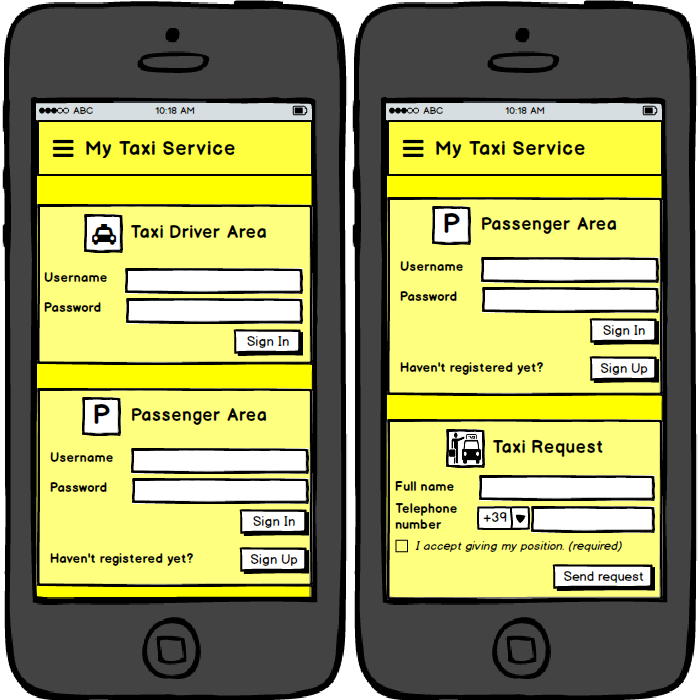
\includegraphics[scale=0.5]{../SE2_MOCKUPS/MobileAppHomePage.png}
				\caption{Home Page - Mobile Application}
				\end{center}	
			\end{figure}
		\end{description}
		
		\newpage
		\paragraph{Home Page - Web Application}
		\begin{figure}[!h]
			\begin{center}					
				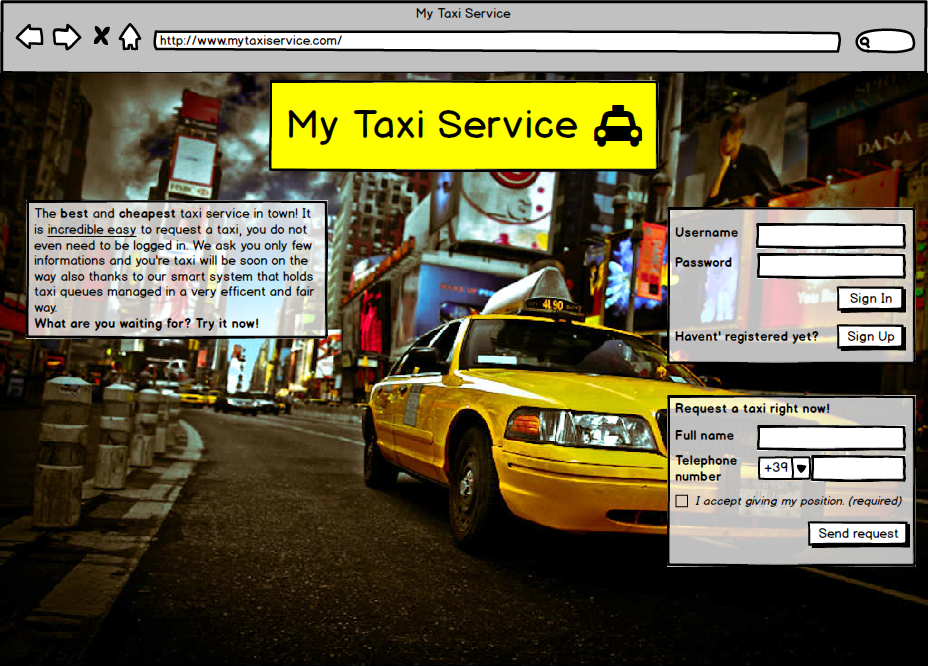
\includegraphics[scale=0.45]{../SE2_MOCKUPS/WebAppHomePage.png}
				\caption{Home Page - Web Application}
			\end{center}	
		\end{figure}
		\newpage
		\paragraph{Registration Form - Mobile Application}
		\begin{figure}[!h]
			\begin{center}
				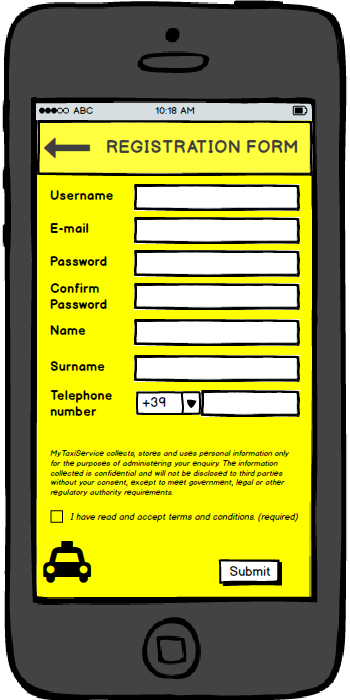
\includegraphics[scale=0.5]{../SE2_MOCKUPS/MobileAppRegistrationForm.png}
				\caption{Registration Form - Mobile Application}	
			\end{center}
		\end{figure}
		\newpage
		\paragraph{Registration Form - Web Application}
		\begin{figure}[!h]
			\begin{center}
				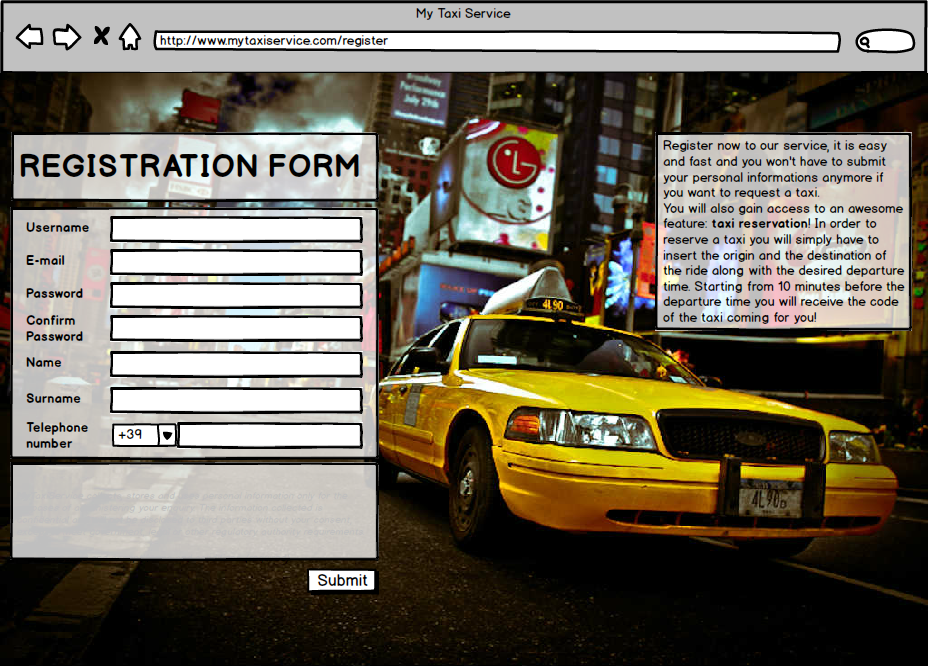
\includegraphics[scale=0.45]{../SE2_MOCKUPS/WebAppRegistrationForm.png}
				\caption{Registration Form -Web Application}	
			\end{center}
		\end{figure}
		\newpage
		\paragraph{Passenger Area - Mobile Application}
		\begin{figure}[!h]
			\begin{center}
				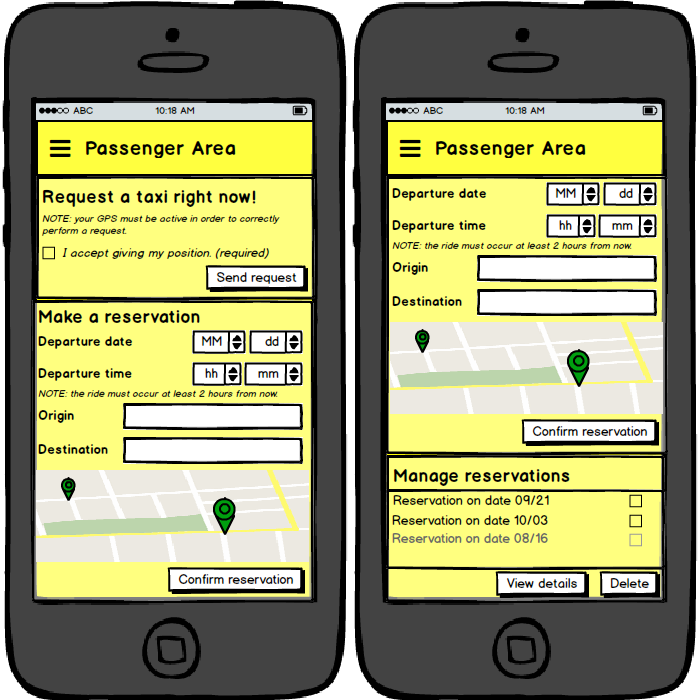
\includegraphics[scale=0.5]{../SE2_MOCKUPS/MobileAppPassengerArea.png}
				\caption{Passenger Area - Mobile Application}
			\end{center}	
		\end{figure}
		\newpage
		\paragraph{Passenger Area - Web Application}
		\begin{figure}[!h]
			\begin{center}
				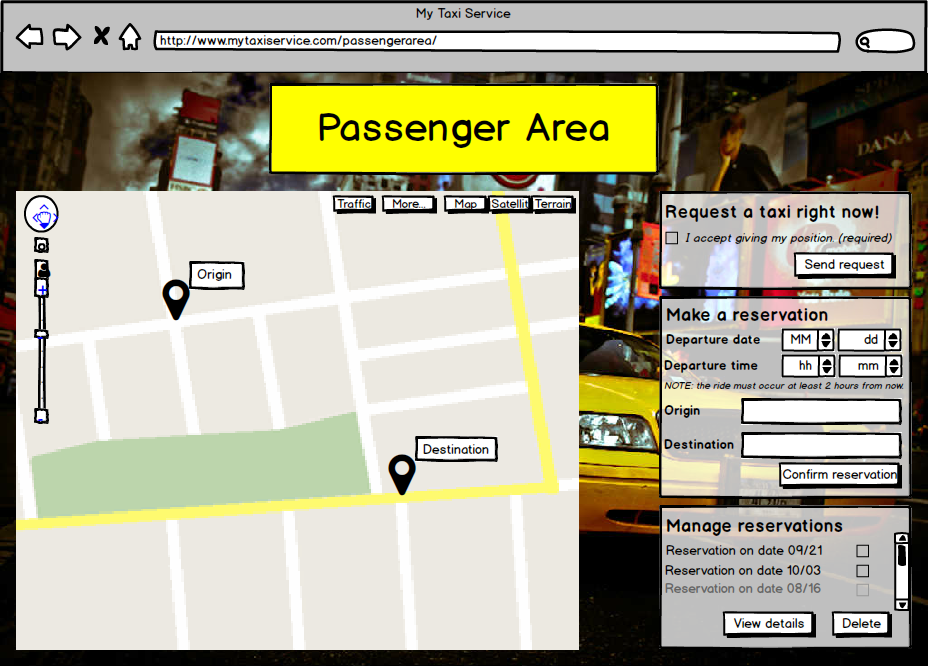
\includegraphics[scale=0.45]{../SE2_MOCKUPS/WebAppPassengerArea.png}
				\caption{Passenger Area - Web Application}
			\end{center}	
		\end{figure}
		\newpage
		\paragraph{Request Confirmation - Mobile Application}
		\begin{figure}[!h]
			\begin{center}
				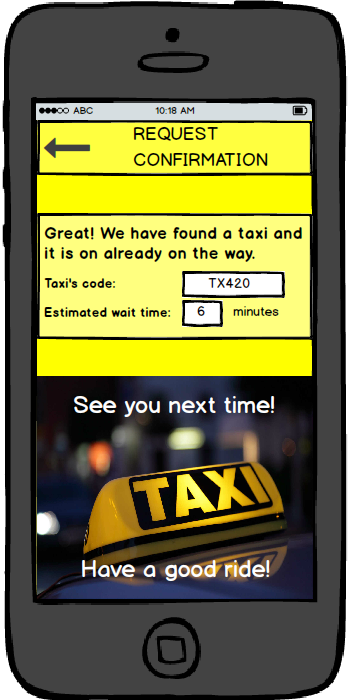
\includegraphics[scale=0.5]{../SE2_MOCKUPS/MobileAppRequestConfirmation.png}
				\caption{Request Confirmation - Mobile Application}
			\end{center}	
		\end{figure}
		\newpage
		\paragraph{Request Confirmation - Web Application}
		\begin{figure}[!h]
			\begin{center}
				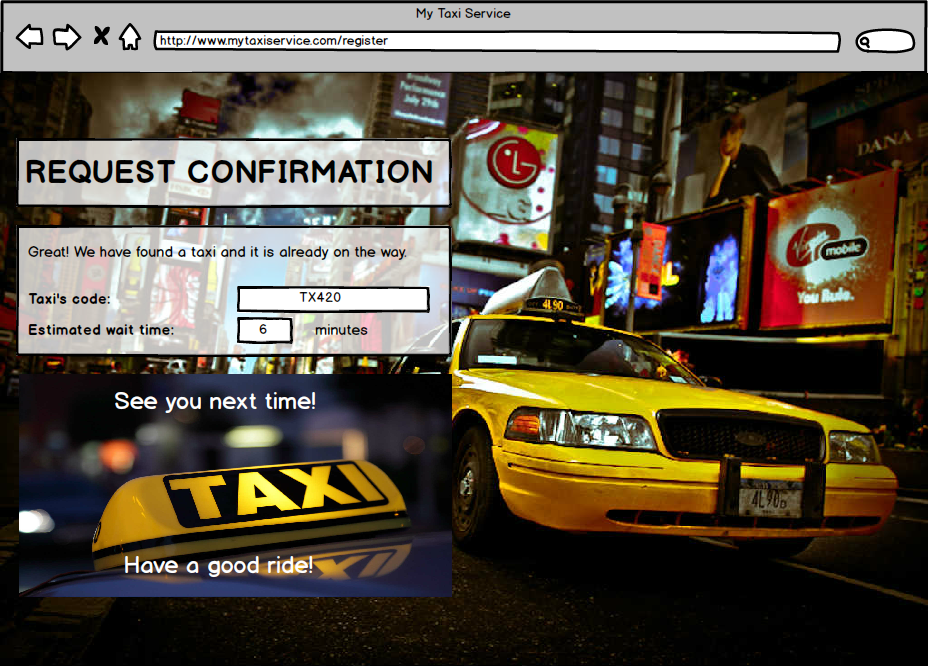
\includegraphics[scale=0.45]{../SE2_MOCKUPS/WebAppRequestConfirmation.png}
				\caption{Request Confirmation - Web Application}
			\end{center}	
		\end{figure}
		\newpage
		\paragraph{Taxi Driver Area - Mobile Application}
		\begin{figure}[!h]
			\begin{center}
				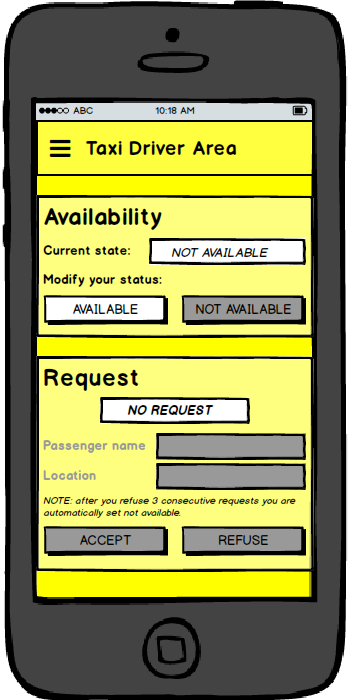
\includegraphics[scale=0.5]{../SE2_MOCKUPS/MobileAppTaxiDriverArea.png}
				\caption{Taxi Driver Area - Mobile Application}	
			\end{center}
		\end{figure}
		\newpage
		\subsubsection{API Interfaces}
			For taxi waiting time and other minor features we decided to use Google Maps API.
			It is a very powerful library that perfectly fits our needs.
			When a taxi accepts a request, the system retrieves its position and, through
			those APIs, is able to process either the hypothetical route that the taxi will
			follow to reach the passenger's position and, consequently, the arrival time.
			The system will, then, forward those information to the passenger.
		\subsubsection{Hardware Interfaces}
			Our project includes a web and a mobile application, so it does not require
			any external hardware interface.
		\subsubsection{Software Interfaces}
			\begin{itemize}
				\item Database Management System (DBMS):
				\begin{itemize}
					\item Name: MySQL.
					\item Version: 5.6.21
					\item Source: http://www.mysql.it/
				\end{itemize}
				\item Java Virtual Machine (JVM).
				\begin{itemize}
					\item Name: JEE
					\item Version: 7
					\item Source: http://www.oracle.com/technetwork/java/javaee/tech/index.html
				\end{itemize}
				\item Application server:
				\begin{itemize}
					\item Name: Glassfish.
					\item Version: 4.1.
					\item Source: https://glassfish.java.net/
				\end{itemize}
				\item Operating System (OS).
				\begin{itemize}
					\item Application must be able to run on any SO which supports JVM and DBMS specified before.
				\end{itemize}
			\end{itemize}
		\subsubsection{Communication Interfaces}
			\begin{center}
				\begin{tabular}{ | l | l | l | p{5cm} |}
					\hline
					Protocol & Application & Port 	\\ \hline
					TCP & HTTPS & 443				\\ \hline
					TCP & HTTP  & 80				\\ \hline
					TCP & DBMS  & 3306 (default)	\\ \hline
				\end{tabular}
			\end{center}
	\subsection{Functional Requirements}
		\subsubsection{Permit a guest to register to the service}
			\begin{enumerate}[label=\bfseries R\arabic*:]
				\item The system shows the registration form to the user when he presses the sign up button.
				\item When the user inserts the username, the email or the phone number, the system verifies that neither of those have already been selected by someone else.
			\end{enumerate}
		\subsubsection{Permit a guest to request a taxi}
			\begin{enumerate}[label=\bfseries R\arabic*:]
				\item The system has to provide a form for storing user basic personal informations.
				\item The system has to ask the user the consensus in order to use his position.
				\item The system has to search for an available taxi in the same area of the user after he presses the request button.
			\end{enumerate}
		\subsubsection{Permit a guest to sign in}
			\begin{enumerate}[label=\bfseries R\arabic*:]
				\item The system has to provide the user a sign in form.
				\item The system, during sign in, verifies that the username and the password inserted by the user have a match in the DB.
			\end{enumerate}
		\subsubsection{Permit a registered passenger to request a taxi}
			\begin{enumerate}[label=\bfseries R\arabic*:]
				\item The system has to ask the user the consensus in order to use his position.
				\item The system has to search for an available taxi in the same area of the user after he presses the request button.
			\end{enumerate}
		\subsubsection{Permit a registered passenger to make a reservation}
			\begin{enumerate}[label=\bfseries R\arabic*:]
				\item User must be already registered and logged in the application.
				\item User must make a reservation at least 2 hours before the request time.
				\item User must provide time, origin and destination of the ride at the moment of the reservation.
				\item User must confirm the reservation process.
				\item The reservation can be deleted by the user himself.
			\end{enumerate}
		\subsubsection{Permit a registered passenger to cancel a reservation}
			\begin{enumerate}[label=\bfseries R\arabic*:]
				\item The system shall check that the passenger is already registered and signed in with
				the correct	credentials.
				\item The system shall check that the request the passenger is deleting, exists and belongs
				to him.
				\item The system shall check that it's not after 10 minutes before the reservation request time.
				\item This process is not reversible
			\end{enumerate}
		\subsubsection{Permit a taxi driver to give the system his availability}
			\begin{enumerate}[label=\bfseries R\arabic*:]
				\item The system shall check that the taxi driver is already registered and signed in with
				the correct	credentials.
				\item The system shall check that the taxi driver is actually unavailable and then
				let the taxi driver set his status as unavailable through the mobile application.
			\end{enumerate}
		\subsubsection{Permit a taxi driver to revoke his availability}
			\begin{enumerate}[label=\bfseries R\arabic*:]
				\item The system shall check that the taxi driver is already registered and signed in with
				the correct	credentials.
				\item The system shall check that the taxi driver is actually available and then
				let the taxi driver set his status as unavailable through the mobile application.
				\item The system shall revoke it automatically if it registers three consecutive request
				rejections.
			\end{enumerate}
		\subsubsection{Permit a taxi driver to accept a ride request}
			\begin{enumerate}[label=\bfseries R\arabic*:]
				\item The system shall check that the taxi driver is already registered and signed in with
				the correct	credentials.
				\item When the system receives a taxi request, it shall remove the first taxi driver
				of that area from the relative queue and notify him, through the mobile application,
				that someone is requesting his taxi.
				\item When the taxi driver receives the notification, he accepts
				\item The system shall register the answer and inform the passenger
				that this taxi is reaching his position.
			\end{enumerate}
		\subsubsection{Permit a taxi driver to refuse a ride request}
			\begin{enumerate}[label=\bfseries R\arabic*:]
				\item The system shall check that the taxi driver is already registered and signed in with
				the correct	credentials.
				\item When the system receives a taxi request, it shall remove the first taxi driver
				of that area from the relative queue and notify him, through the mobile application,
				that someone is requesting his taxi.
				\item When the taxi driver receives the notification, he declines the request.
				\item If this taxi driver is at the third consecutive rejection, the system shall set his status as unavailable,
				notifying him
				\item If this taxi driver is at the first or second consecutive rejection, the system shall put him
				at the end of his area queue.
			\end{enumerate}
	\subsection{Scenarios}
		\subsubsection{Occasional user}
			Mario, an important businessman, has just arrived by train in our city for the first time.
			His train had technical issues and now he is a bit late for the meeting on 
			the opposite side of the town, so he does not want to take public transports.
			The best solution is to call a taxi.
			He opens the browser on his smartphone and, inserting name, surname and his telephone number, sends a taxi request
			to our system. As soon as possible he receives a notification with the taxi ID number and the
			waiting time before the taxi arrival. Mario manages to get there sooner than expected thanks to our service.
		\subsubsection{Habitual user}
			The meeting of Mario went very well: he started an important collaboration with a local
			company. He will have to come back often in our town. He found our service very useful, so
			he decides to download our mobile application and sign up to the service. After a couple of weeks he has to
			come back. Unfortunately his train had technical issues, and he risks to be late to the
			meeting again. This time he has our application installed on his mobile device, so with only
			few taps and no additional information needed, requests a taxi. As soon as possible he receives
			a notification with the taxi ID number and the	waiting time before the taxi arrival.
			Once again our service saves his day.
		\subsubsection{Taxi reservation}
			After another couple of weeks, Mario has to come back in our town again. He thinks that he 
			will never be so unlucky to find a defective train for the third consecutive time,
			so he decides to make a reservation before leaving his place,in order to find a taxi waiting for him
			at the train station at his arrival. Using the mobile application, he fills in all the
			necessary fields, indicating hour and place of the request.
			Now he can enjoy his journey carefree.
		\subsubsection{Deleting a taxi reservation}
			Mario's train has technical issues. Poor Mario, he's so unlucky! He will be very late, 
			so he does not want to let the taxi wait so long. He opens our application and, 30 minutes
			before the taxi request, he selects the reservation and deletes it. Once arrived he will
			request a taxi as usual.
		\subsubsection{Taxi driver}
			A taxi driver, Luigi, is having a little break, eating his favourite chocolate bar in his taxi. Suddenly
			his phone rings: a notification has just arrived. But he's having a break, so he does not answer.
			After 1 minute, the system automatically records a negative answer.
			Luigi slowly ends his bar and starts answering some messages on his smartphone. Suddenly his phone
			rings. He sees another notification, but he's very busy, so he declines the request. Luigi greets his
			friend on the chat and goes back to work. After a few minutes his phone rings again. A man called
			Mario is requesting a taxi in his area, right next to the train station. He accepts the request and
			starts driving towards the location of the customer.
		\subsubsection{Taxi availability}
			After a hard morning, Luigi decides that it is the right time to have lunch. He opens our mobile
			application and sets his status to unavailable: he does not want to be disturbed during such an
			important moment. After lunch, he goes back to work, so he picks up his phone, opens our
			application and sets his status to available. He works hard for the whole afternoon and, after the
			last passenger, he's so tired that he forgets the status on available. The system sends him 1, 2, 3
			notifications of requests, but Luigi has a huge headache and can not hear the phone ringing. After
			the third request without answer the system automatically sets his status to unavailable.
			Finally Luigi will get its deserved peace.
	\newpage
	\subsection{UML models}
		\subsubsection{Use Case diagram}
			\begin{figure}[h!]
				\centering
				\graphicspath{ {../SE2_IMAGES/} }
				\includegraphics[height=0.8\textheight]{UseCase.png}
				\caption{Use Case Diagram for MyTaxiService}
			\end{figure}
		\newpage
		\subsubsection{Class diagram}
			\begin{figure}[h!]
				\centering
				\graphicspath{ {../SE2_IMAGES/} }
				\includegraphics[width=\linewidth]{ClassDiagram.png}
				\caption{Class Diagram for MyTaxiService}
			\end{figure}
		\paragraph{Guest Registration}
			\begin{center}
				\begin{tabular}{ | l | p{8cm} |}
					\hline
					Actor &  Guest	\\ \hline
					Preconditions & The guest has not registered yet to the service		\\ \hline
					Execution Flow & \begin{enumerate}
						\item The guest presses the sign up button and access the registration form
						\item The form requires to insert username, email, password, password confirmation, name, surname, telephone number and to accept terms and conditions
						\item The system verifies that username, email and telephone number are uniques
						\item The system confirms the registration
						\item The system automatically loads the Passenger Area page
					\end{enumerate}		\\ \hline
					Postconditions & The guest is now a Registered Passenger and is logged in to the service	\\ \hline
					Exceptions & Username, password or email are not uniques; the registration fails \\ \hline
				\end{tabular}
			\end{center}
			\begin{figure}[!h]
				\begin{center}			
					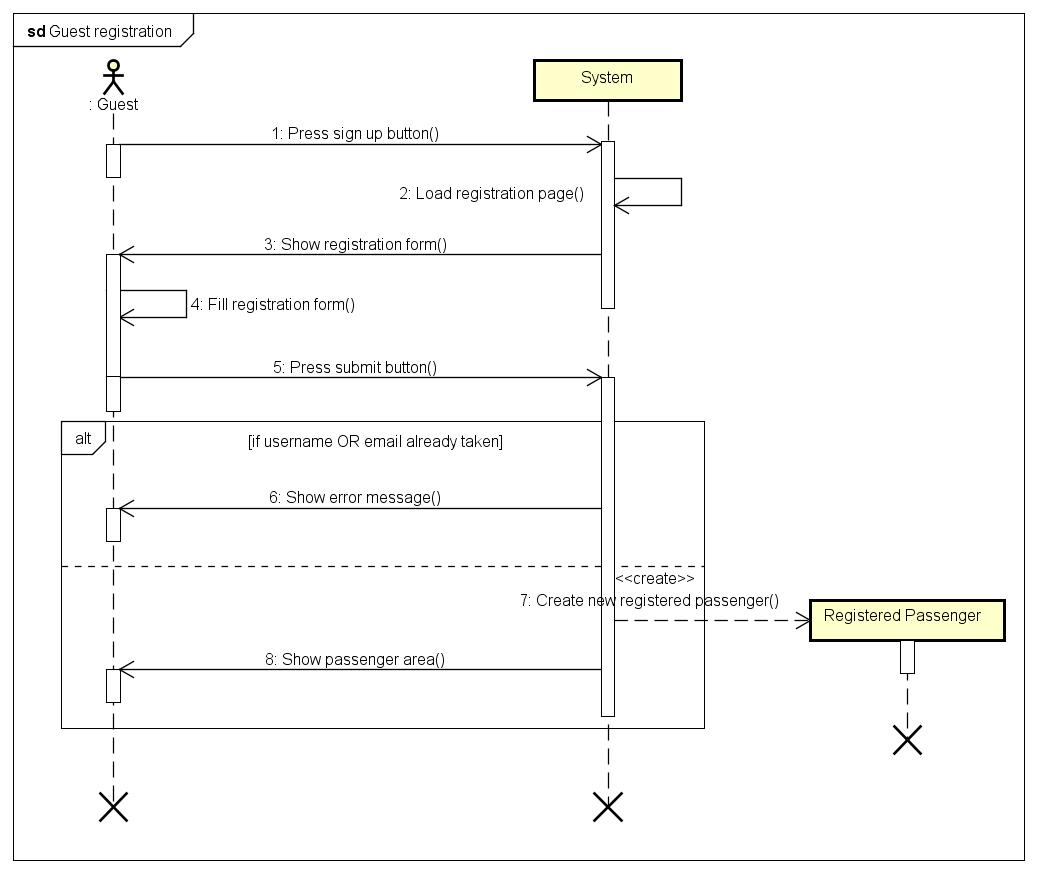
\includegraphics[scale=0.45]{../SE2_SD/GuestRegistration}
					\caption{Sequence Diagram - Guest Registration}	
				\end{center}
			\end{figure}
		\paragraph{Registered Passenger Sign In}
			\begin{center}
				\begin{tabular}{ | l | p{8cm} |}
					\hline
					Actor &  Registered Passenger	\\ \hline
					Preconditions & The registered passenger is registered to the service	\\ \hline
					Execution Flow & \begin{enumerate}
						\item The registered passenger fills the sign in form, which requires to insert username and password
						\item The guest presses the sign in
						\item The system verifies that username and password matches
						\item The system loads the Passenger Area page
					\end{enumerate}		\\ \hline
					Postconditions & The registered passenger is logged in to the service	\\ \hline
					Exceptions & Username not existent or username-password mismatch; the sign in fails \\ \hline
				\end{tabular}
			\end{center}
			\begin{figure}[!h]
				\begin{center}			
				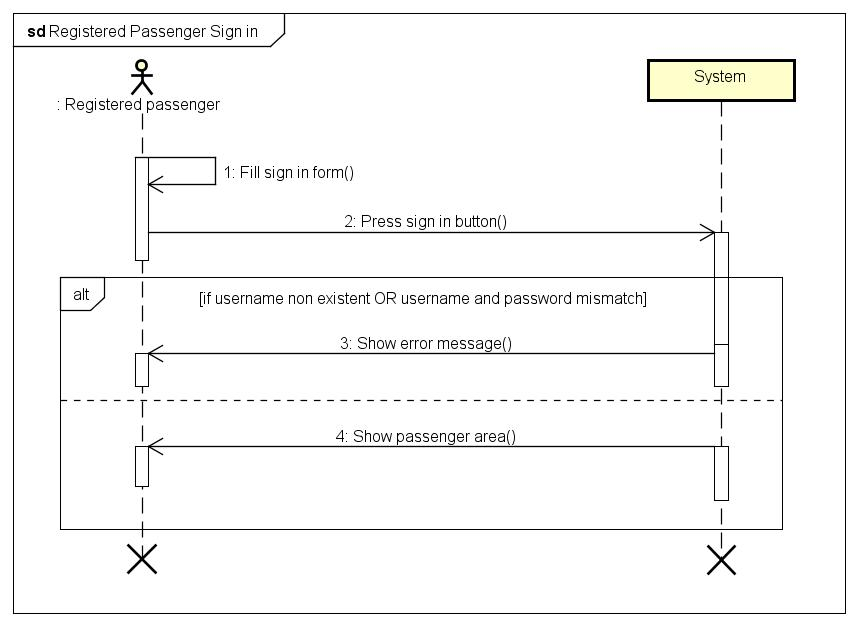
\includegraphics[scale=0.5]{../SE2_SD/RegisteredPassengerSignIn}
				\caption{Sequence Diagram - Registered Passenger Sign In}	
				\end{center}
			\end{figure}
		\paragraph{Guest Taxi Request}
			\begin{center}
				\begin{tabular}{ | l | p{8cm} |}
					\hline
					Actor &  Guest	\\ \hline
					Preconditions & Nothing		\\ \hline
					Execution Flow & \begin{enumerate}
						\item The guest fills the request form, which requires to insert full name and telephone number and to give position consensus
						\item The guest presses the request button
						\item The system searches and finds an available taxi
						\item The system loads the confirmation request page
					\end{enumerate}		\\ \hline
					Postconditions & The Guest has the code of the taxi he requested	\\ \hline
					Exceptions & GPS position not available; the request fails \\ \hline
				\end{tabular}
			\end{center}
			\begin{figure}[!h]
				\begin{center}			
					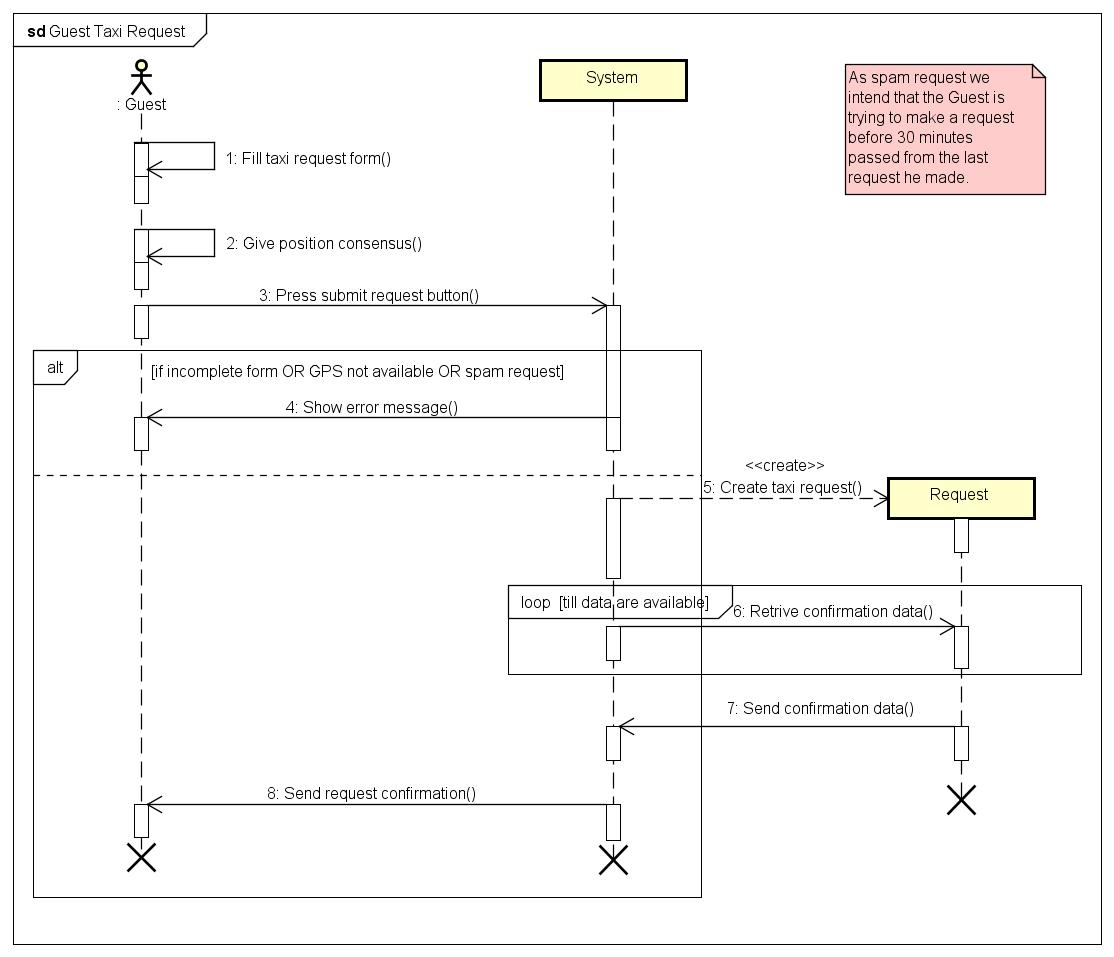
\includegraphics[scale=0.4]{../SE2_SD/GuestTaxiRequest}
					\caption{Sequence Diagram - Guest Taxi Request}	
				\end{center}
			\end{figure}
		\paragraph{Registered Passenger Taxi Request}
			\begin{center}
				\begin{tabular}{ | l | p{8cm} |}
					\hline
					Actor &  Registered Passenger	\\ \hline
					Preconditions & The registered passenger is registered to the service	\\ \hline
					Execution Flow & \begin{enumerate}
						\item The registered passenger signs in to the service (as written above) and access the Passenger Area page
						\item The registered passenger gives position consensus and presses the request button
						\item The system searches and finds an available taxi
						\item The system loads the confirmation request page
					\end{enumerate}		\\ \hline
					Postconditions & The registered passenger has the code of the taxi he requested	\\ \hline
					Exceptions & GPS position not available; the request fails \\ \hline
				\end{tabular}
			\end{center}
			\begin{figure}[!h]
				\begin{center}			
					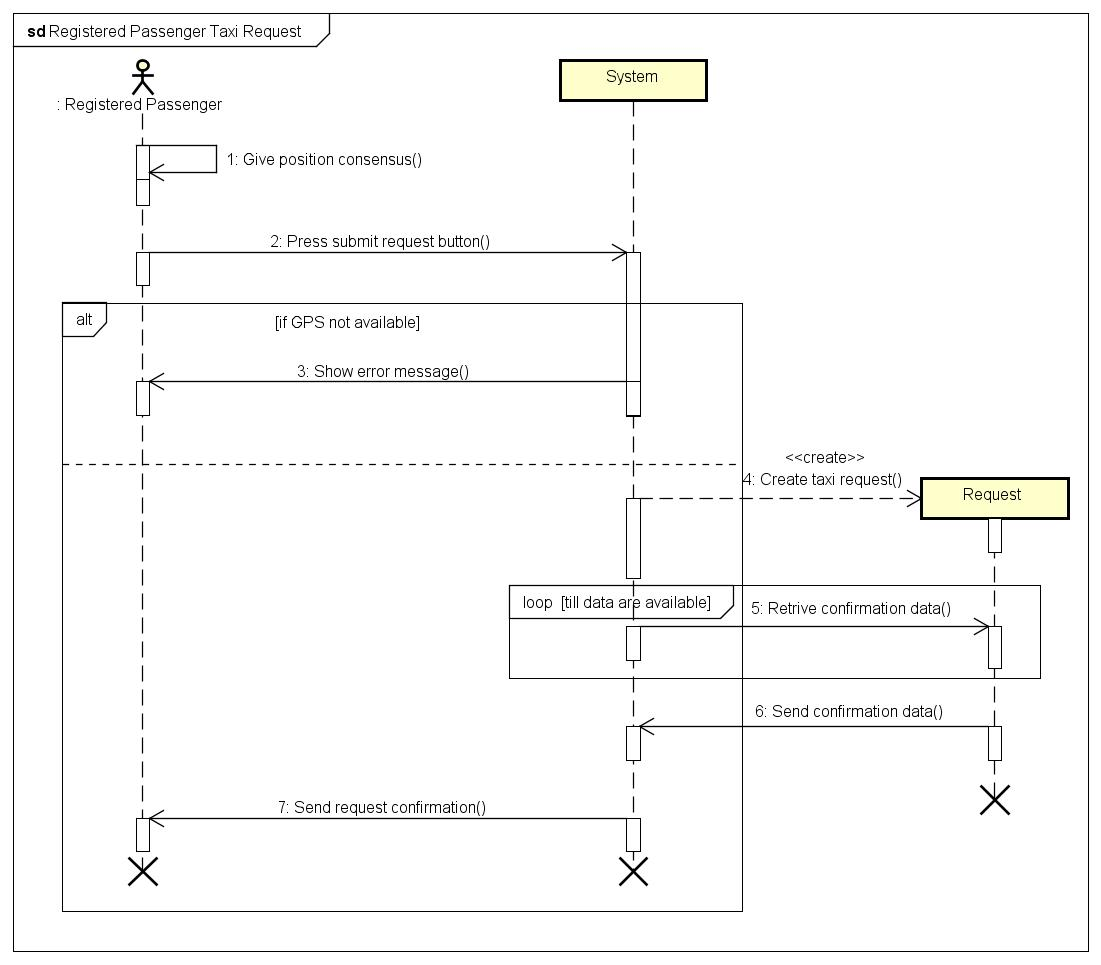
\includegraphics[scale=0.4]{../SE2_SD/RegisteredPassengerTaxiRequest}
					\caption{Sequence Diagram - Registered Passenger Taxi Request}	
				\end{center}
			\end{figure}
		\paragraph{Cancel a reservation}
			\begin{center}
				\begin{tabular}{ | l | p{8cm} |}
					\hline Actors & Registered passenger
					\\ \hline
					Preconditions &
					The user is logged into the system as registered passenger and has already made
					a reservation
					\\ \hline
					Execution Flow &
					\begin{enumerate}
						\item The user accesses his personal page with the list of reservations
						\item The user selects the reservation that wants to delete and presses the apposite
						button
						\item The system cancels his reservation and reloads the Passenger Area page
					\end{enumerate}
					\\ \hline
					Postconditions & The reservation is cancelled and no requests will be forwarded
					\\ \hline
					Exceptions &
					It's too late to cancel the reservation (after 10 minutes before the time established):
					the reservation is not cancelled and the user is notified.
					\\ \hline
				\end{tabular}
			\end{center}
		\paragraph{Give availability}
			\begin{center}
				\begin{tabular}{ | l | p{8cm} |}
					\hline Actors & Taxi driver
					\\ \hline
					Preconditions &
					The user is logged into the system as taxi driver and is using the mobile application
					\\ \hline
					Execution Flow &
					\begin{enumerate}
						\item The taxi driver accesses his personal area
						\item The taxi driver presses the apposite button
						\item The system sets the taxi driver status as available
						\item The system inserts the taxi driver in his area queue
					\end{enumerate}
					\\ \hline
					Postconditions & 
					The taxi driver is now available and will receive notifications of taxi requests.
					\\ \hline
					Exceptions &
					The taxi driver is already available: the system will not react anyway at the button
					pressure.
					\\ \hline
				\end{tabular}
			\end{center}
		\paragraph{Revoke availability}
			\begin{center}
				\begin{tabular}{ | l | p{8cm} |}
					\hline Actors & Taxi driver
					\\ \hline
					Preconditions &
					The user is logged into the system as taxi driver and is using the mobile application
					\\ \hline
					Execution Flow &
					\begin{enumerate}
						\item The taxi driver accesses his personal area
						\item The taxi driver presses the apposite button
						\item The system sets the taxi driver status as unavailable
						\item The system removes the taxi driver from his area queue
					\end{enumerate}
					\\ \hline
					Postconditions & 
					The taxi driver is now unavailable and will not receive notifications of taxi requests.
					\\ \hline
					Exceptions &
					The taxi driver is already unavailable: the system will not react anyway at the button
					pressure.
					\\ \hline
				\end{tabular}
			\end{center}
		\paragraph{Accept a ride request}
			\begin{center}
				\begin{tabular}{ | l | p{8cm} |}
					\hline Actors & Taxi driver
					\\ \hline
					Preconditions &
					The user is logged into the system as taxi driver and is using the mobile application
					\\ \hline
					Execution Flow &
					\begin{enumerate}
						\item The taxi driver receives the notification of a request
						\item The taxi driver accesses his personal page
						\item The taxi driver presses the Accept button
						\item The system notifies the user who asked for the taxi sending him
						information about the taxi and the arrival time
					\end{enumerate}
					\\ \hline
					Postconditions & The taxi driver is not enqueued again and the user's request
					is considered satisfied
					\\ \hline
					Exceptions &
					The taxi driver does not answer within 1 minute:
					the system automatically records a rejection.
					\\ \hline
				\end{tabular}
			\end{center}
		\paragraph{Refuse a ride request}
			\begin{center}
				\begin{tabular}{ | l | p{8cm} |}
					\hline Actors & Taxi driver
					\\ \hline
					Preconditions &
					The user is logged into the system as taxi driver and is using the mobile application
					\\ \hline
					Execution Flow &
					\begin{enumerate}
						\item The taxi driver receives the notification of a request
						\item The taxi driver accesses his personal page
						\item The taxi driver presses the Decline button
						\item The system records the rejection and reinserts the taxi at the end of
						the area queue
						\item The system sends the request notification to another taxi
					\end{enumerate}
					\\ \hline
					Postconditions & The taxi driver is enqueued again and the user's request
					is considered unsatisfied
					\\ \hline
					Exceptions &
					The taxi driver does not answer within 1 minute:
					the system automatically records a rejection.
					The taxi driver is at the third consecutive rejection:
					the system does not enqueue the taxi driver and sets his status as unavailable
					\\ \hline
				\end{tabular}
			\end{center}
\section{Alloy Modelling}
	In this chapter the consistency of the proposed Class Diagram will be
	tested via Alloy Analyzer. The report that follow is composed by the code
	used to describe the model and an example of world generated by our predicates.
	\subsection{Alloy Code}
	\lstset{language=Alloy}
	\begin{lstlisting}
module MyTaxiService

/*** Class declaration ***/
open util/boolean

sig GenericText{}

sig GenericData{
year: one Int,
month: one Int,
day: one Int,
hour: one Int,
minute: one Int
}{
year > 0 and
month > 0 and
day > 0 and
hour > 0 and
minute > 0
}

sig Guest {
ip: one GenericText
--name: one GenericText,
--surname: one GenericText,
--telephone: one GenericText
}

sig RegisteredPassenger extends Guest{
username: one GenericText,
email: one GenericText,
--password: one GenericText,
}

sig TaxiDriver{
taxiID: one GenericText,
availability: one Bool
--name: one GenericText,
--surname: one GenericText
}

sig Request{
area: one Area,
passenger: one Guest,
when: one GenericData
}

sig Reservation{
passenger: one RegisteredPassenger,
area: one Area,
when: one GenericData
}

sig Area {
where: one GenericText,
queue: set TaxiDriver
}

-- there are also other attributes but are not relevants for this representation

/*** DEFINITION OF THE CONSTRAINTS ***/

--each email has to be unique
fact emailUnicity{
no disj rp1, rp2: RegisteredPassenger | rp1.email = rp2.email
}

--each username has to be unique
fact usernameUnicity{
no disj rp1, rp2: RegisteredPassenger | rp1.username = rp2.username
}

--each taxiID has to be unique
fact taxiIDUnicity{
no disj t1, t2: TaxiDriver | t1.taxiID = t2.taxiID
}

--each Area has to be unique
fact areaUnicity{
no disj a1, a2: Area | a1.where = a2.where
}

--each taxi, if available, must be in only one queue
fact onlyOneTaxi{
all t: TaxiDriver | t.availability = True implies one a: Area | t in a.queue
}

--each taxi, if not available, must not be in any queue
fact noOneTaxi{
all t: TaxiDriver | t.availability = False implies all a: Area | t not in a.queue
}

--a user can not have two requests without 30 minutes of distance betweeen them
fact requestTime{
all disj r1, r2: Request |
r1.when.year = r2.when.year and
r1.when.month= r2.when.month and
r1.when.day= r2.when.day and
r1.when.hour= r2.when.hour and
r1.when.minute > r2.when.minute and
r1.when.minute - r2.when.minute < 30 implies r1.passenger != r2.passenger
}

--the same passenger can't have two reservation with desired time within 30 minutes from one another
fact reservationTime{
all disj r1, r2: Reservation |  
r1.when.year = r2.when.year and
r1.when.month= r2.when.month and
r1.when.day= r2.when.day and
r1.when.hour= r2.when.hour and
r1.when.minute > r2.when.minute and
r1.when.minute - r2.when.minute < 30 implies r1.passenger != r2.passenger
}

/*** FUNCTION ***/

fun passengerRequests [g: Guest]: set Request{
{r: Request | g = r.passenger}
}

fun passengerReservations [p: RegisteredPassenger]: set Reservation{
{r: Reservation | p = r.passenger}
}

fun getTaxiAreas [t: TaxiDriver]: set Area{
{a: Area | t in a.queue}
}

/*** ASSERTION ***/

--check that a taxi is in a sngle queue or is not in any
assert oneTaxiOneQueue{
all t: TaxiDriver | #getTaxiAreas[t] <= 1
}

check oneTaxiOneQueue for 3


--the same registered passenger doesn't have two reservations with desired time within 30 minutes from one another
assert noSpamReservation{
all p: RegisteredPassenger | no disj r1, r2: Reservation | r1 in passengerReservations [p] and r2 in passengerReservations [p] and 
r1.when.year = r2.when.year and
r1.when.month= r2.when.month and
r1.when.day= r2.when.day and
r1.when.hour= r2.when.hour and
r1.when.minute < r2.when.minute and
r1.when.minute - r2.when.minute < 30
}

check noSpamReservation for 3

--the same passenger doesn't have two requests within 30 minutes from one another
assert noSpamRequest{
all g: Guest | no disj r1, r2: Request | r1 in passengerRequests[g] and r2 in passengerRequests[g] and 
r1.when.year = r2.when.year and
r1.when.month= r2.when.month and
r1.when.day= r2.when.day and
r1.when.hour= r2.when.hour and
r1.when.minute > r2.when.minute and
r1.when.minute - r2.when.minute < 30
}

check noSpamRequest for 3

/*** PREDICATES ***/

pred hardSituation{
#Guest  > 10 and
#RegisteredPassenger > 10 and
#TaxiDriver > 5 and
#Request > 5 and
#Reservation > 2
}

run hardSituation for 20

pred casualSituation{
#Guest  > 1 and
#RegisteredPassenger > 1 and
#TaxiDriver > 1 and
#Request > 1
}

run casualSituation for 3

pred show{

}

run show for 2

	\end{lstlisting}
	\newpage
	\subsection{Alloy Response}
	
	Here the alloy response for the model is shown.
	
	\begin{figure}[!h]
		\begin{center}			
			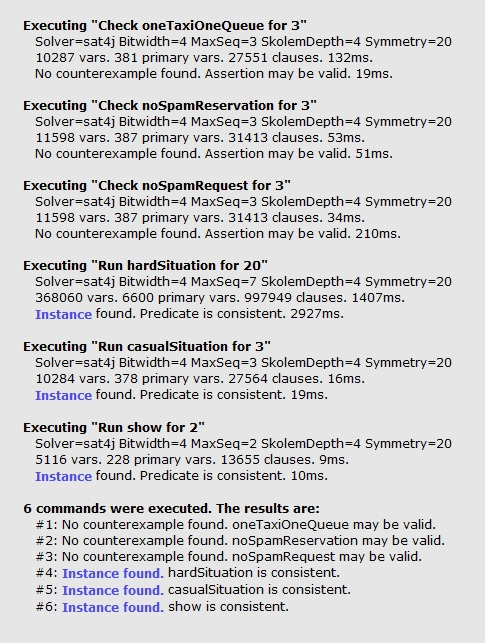
\includegraphics[scale=1]{../SE2_ALLOY/Answer}
			\caption{Alloy Answer}	
		\end{center}
	\end{figure}
	
	\subsection{Alloy Worlds}
		\subsubsection{Hard Situation}
		We do not insert the image for this test case because is huge and
		pretty incomprehensible. The test has been executed to ensure that the
		model keeps its consistency also with a significant number of entities.
		\newpage
		\begin{landscape}
		\subsubsection{Casual Situation}
		Here is shown the world generated by Alloy Analizer via the
		execution of the predicate "casualSituation".
		We have added basic constraints to this predicate, in order to ensure
		that everything has at least an instance (until a maximum of 3).
		The reservation is not considered because it's an advanced feature and
		has been tested deeply in the hard situation. However the system added
		an instance automatically.
			\begin{figure}[!h]
				\begin{center}			
					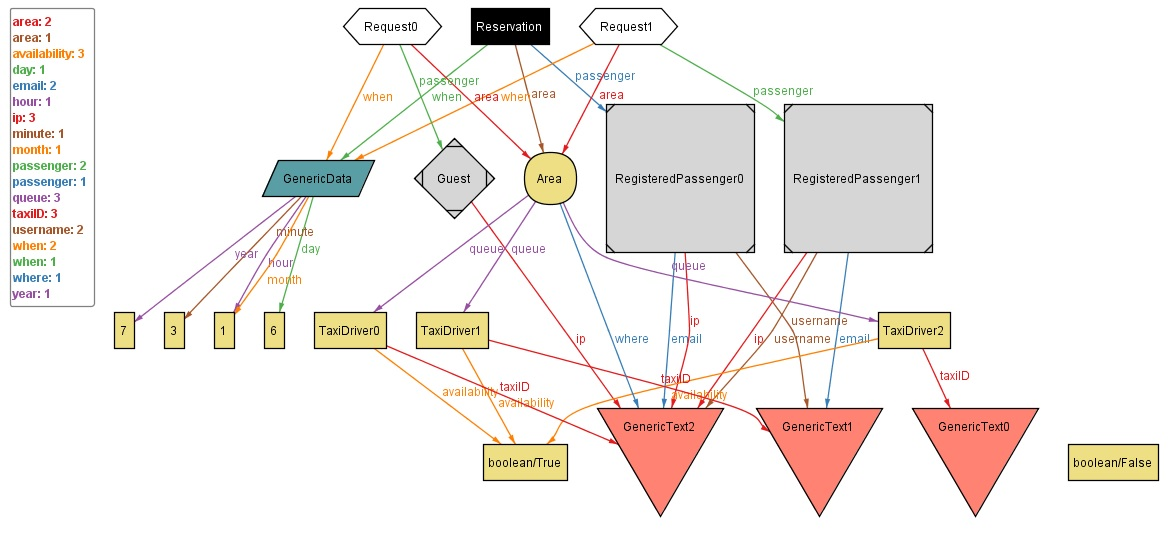
\includegraphics[height=0.65\textheight]{../SE2_ALLOY/CasualSituation}
					\caption{World Representation - Casual Situation}	
				\end{center}
			\end{figure}
		\end{landscape}
		\newpage
		\begin{landscape}
		\subsubsection{Show}
		Here is shown the world generated by Alloy Analizer via the
		execution of the predicate "show".
		In this predicate there are no constraints.
		The predicate generates a world that respects the given constraints where
		each entities has at maximum 2 instances (to keep the representation
		model little and readable).
			\begin{figure}[!h]
				\begin{center}			
					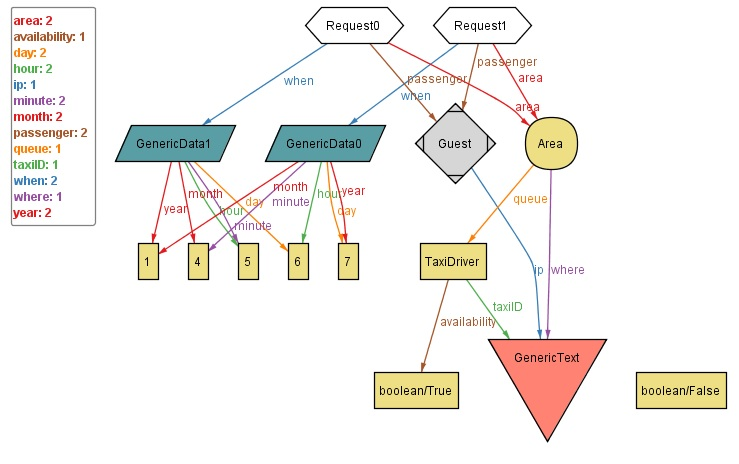
\includegraphics[height=0.65\textheight]{../SE2_ALLOY/Show}
					\caption{World Representation - Default Show}	
				\end{center}
			\end{figure}
		\end{landscape}
\section{Other Info}
\subsection{Hours of work}
	For each component follows an approximate indication of how much time was
	spent on the realization of this document
	\begin{center}
		\begin{tabular}{ | l | l | p{5cm} |}
			\hline
			Component & Hours 					\\ \hline
			Bernardis Cesare & 32 				\\ \hline
			Dagrada Mattia & 30  				\\ \hline
			\end{tabular}
			\end{center}
			
\subsection{Tools}
	We used various tools to develop this document:
	\begin{itemize}
		\item \LaTeXe \, and TeXMaker editor 2.10.4
		\item Astah Professional 7.0.0
		\item Draw.IO
	\end{itemize}

\subsection{Version 2.0}
We changed few things in the interfaces section since some functionalities were 
assigned to the wrong interface.  

\end{document}